% Options for packages loaded elsewhere
\PassOptionsToPackage{unicode}{hyperref}
\PassOptionsToPackage{hyphens}{url}
%
\documentclass[
  11pt,
]{article}
\usepackage{lmodern}
\usepackage{setspace}
\usepackage{amssymb,amsmath}
\usepackage{ifxetex,ifluatex}
\ifnum 0\ifxetex 1\fi\ifluatex 1\fi=0 % if pdftex
  \usepackage[T1]{fontenc}
  \usepackage[utf8]{inputenc}
  \usepackage{textcomp} % provide euro and other symbols
\else % if luatex or xetex
  \usepackage{unicode-math}
  \defaultfontfeatures{Scale=MatchLowercase}
  \defaultfontfeatures[\rmfamily]{Ligatures=TeX,Scale=1}
\fi
% Use upquote if available, for straight quotes in verbatim environments
\IfFileExists{upquote.sty}{\usepackage{upquote}}{}
\IfFileExists{microtype.sty}{% use microtype if available
  \usepackage[]{microtype}
  \UseMicrotypeSet[protrusion]{basicmath} % disable protrusion for tt fonts
}{}
\usepackage{xcolor}
\IfFileExists{xurl.sty}{\usepackage{xurl}}{} % add URL line breaks if available
\IfFileExists{bookmark.sty}{\usepackage{bookmark}}{\usepackage{hyperref}}
\hypersetup{
  hidelinks,
  pdfcreator={LaTeX via pandoc}}
\urlstyle{same} % disable monospaced font for URLs
\usepackage[margin=1in]{geometry}
\usepackage{graphicx,grffile}
\makeatletter
\def\maxwidth{\ifdim\Gin@nat@width>\linewidth\linewidth\else\Gin@nat@width\fi}
\def\maxheight{\ifdim\Gin@nat@height>\textheight\textheight\else\Gin@nat@height\fi}
\makeatother
% Scale images if necessary, so that they will not overflow the page
% margins by default, and it is still possible to overwrite the defaults
% using explicit options in \includegraphics[width, height, ...]{}
\setkeys{Gin}{width=\maxwidth,height=\maxheight,keepaspectratio}
% Set default figure placement to htbp
\makeatletter
\def\fps@figure{htbp}
\makeatother
\setlength{\emergencystretch}{3em} % prevent overfull lines
\providecommand{\tightlist}{%
  \setlength{\itemsep}{0pt}\setlength{\parskip}{0pt}}
\setcounter{secnumdepth}{-\maxdimen} % remove section numbering

\author{}
\date{\vspace{-2.5em}}

\begin{document}

\setstretch{1.25}
\clearpage

\hypertarget{fundamentauxe7uxe3o-teuxf3rica}{%
\section{1. Fundamentação
teórica}\label{fundamentauxe7uxe3o-teuxf3rica}}

\hypertarget{mudanuxe7as-climuxe1ticas-alterauxe7uxe3o-na-distribuiuxe7uxe3o-de-espuxe9cies-e-mismatch-espacial}{%
\subsection{\texorpdfstring{1.1 Mudanças climáticas, alteração na
distribuição de espécies e \emph{mismatch}
espacial}{1.1 Mudanças climáticas, alteração na distribuição de espécies e mismatch espacial}}\label{mudanuxe7as-climuxe1ticas-alterauxe7uxe3o-na-distribuiuxe7uxe3o-de-espuxe9cies-e-mismatch-espacial}}

~~~~~A distribuição de uma espécie se caracteriza pela área geográfica a
qual ela pode ser encontrada {[}@putten2012{]}, o que é estabelecido por
uma série de fatores determinados pelo nicho ecológico da espécie
{[}@begon2005{]}. Ao serem afetadas por transformações do clima, a
população de uma espécie pode ter três desfechos possíveis: adaptação às
novas condições, extinção local ou migração para novos ambientes
adequados à sobrevivência da espécie {[}@parmesan2006;
@gorostiague2018{]}.

Diversas observações de alterações na distribuição de espécies em
paralelo às mudanças climáticas (tratado aqui principalmente como o
aquecimento do clima global) já foram documentadas ao redor do globo
{[}@parmesan2003; @walther2002{]}. Essas alterações podem ter escalas
muito distintas entre as espécies, algumas podem ter repostas evolutivas
adequadas quanto às mudanças na distribuição devido ao aquecimento do
clima {[}@chen2011{]}, enquanto que outras tendem a não responder de
maneira adequada e acabarem extintas localmente {[}@parmesan2006{]}.

Embora as respostas evolucionárias de alteração na distribuição tenham
proporções distintas, observa-se uma tendência de muitas espécies a
mudarem suas distribuições em direção altitudes maiores e latitudes
polares {[}@chen2011, @parmesan2003; @parmesan2006{]}. Nas regiões
tropicais, espécies seguem a mesma tendência ao movimento para áreas
mais temperadas {[}@parmesan2006{]}.

Além do mais, tem sido indicado que as mudanças climáticas podem
pertubar interações ecológicas entre espécies, podendo levar ao chamado
\emph{mismatch} espacial (ruptura ou diminuição das interações
ecológicas em razão do desencontro geográfico das espécies)
{[}@schweiger2008; @hegland2008{]}. Pelas respostas evolutivas às
mudanças climáticas não acontecerem de formas iguais é que ocorrem os
\emph{mismatches}. @gorostiague2018 apontou que as chances que a
população de uma espécie tem de colonizar novos habitats depende da
possibilidade de que as espécies das quais ela dependa também expandam
sua distribuição (\emph{match} espacial com seus parceiros mutualistas),
caso o contrário ocorrerá o \emph{mismatch} espacial.

No caso de sistemas ecológicos planta-polinizador, há uma grande
preocupação em compreender como as mudanças climáticas podem afetar as
distribuições de plantas e seus polinizadores e também os impactos dos
\emph{mismatches} sobre os mesmos, tendo em vista a contribuição
ambiental desses sistemas e o papel ecológico nos ecossistemas
{[}@begon2005; @ke arns1998{]}.

Para as plantas, o \emph{mismatch} com polinizadores efetivos poderia
causar a redução da deposição do pólen, aumentando a restrição deste,
segundo @hegland2008. É comum em diversas espécies de plantas a
limitação da reprodução devido a polinização insuficiente, conhecido
como \emph{Efeito Allee}. Quanto aos polinizadores, pode-se esperar que
o desencontro com plantas importantes à alimentação leve a uma redução
na quantidade e acesso a alimentos, afetando diretamente sua
sobrevivência. @hegland2008 também discute que os efeitos dos
\emph{mismatches} podem ser mais rigoroso aos polinizadores, pois a
dependência dos polinizadores na nutrição é maior do que a dependência
das plantas que florescem na polinização. Contudo, a força com que
espécies de polinizadores são afetados pelos \emph{mismatches} pode
depender dos traços funcionais (características fisiológicas,
fenológicas e morfológicas) das espécies, como no caso de morcegos
polinizadores {[}@gutierrez2021{]}.

\begin{figure}
\centering
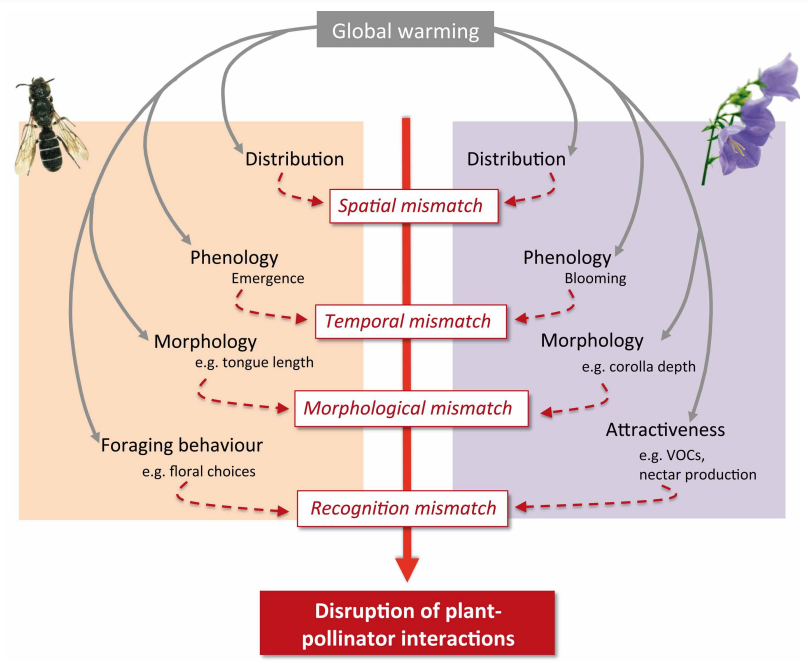
\includegraphics[width=0.6\textwidth,height=\textheight]{mismatch.png}
\caption{Possíveis impactos dos \emph{mismatches} (espacial, temporal,
morfológico e de reconhecimento) nas interações entre plantas e
polinizadores. Imagem retirada da fonte: @gerard2020}
\end{figure}

Apesar dos possíveis efeitos negativos causados pelos \emph{mismatches},
algumas características de muitos sistemas planta-polinizador podem agir
para minimizar os impactos, como a estrutura aninhada de redes de
polinização, na qual um núcleo de espécies generalistas interagem entre
si e as espécies especilistas dessa rede interagem apenas com as
generalistas {[}@hegland2008; @jordano2003{]}. Ademais, há mais espécies
generalistas nessas redes do que especialistas, sendo que relações de um
único polinizador para uma planta são incomuns, o que pode contribuir
para que muitas espécies não sejam afetadas gravemente pelos
\emph{mismatches}. Por fim, a maioria das interações de polinização são
assimétricas, isto é, caso uma planta seja importante para um
polinizador, então a importância desse polinizador para a planta é baixa
{[}hegland2008; @gutierrez2021{]}.

Por mais que essas propriedades das redes de polinização possam atuar
como estabilizadores diante de distúrbios, as redes de polinização ainda
podem ser enfraquecidas pelos impactos negativos dos \emph{mismatches}.
Tem sido proposto que em sistemas nos quais interações são formadas por
generalistas, os polinizadores mostrem maior plasticidade para se
adequar às mudanças, enquanto que em sistemas com espécies especialistas
exista menor flexibilidade nas respostas, estando portanto mais
vulneráveis {[}@memmott2007; @rafferty2012{]}. Espécies com distribuição
restrita também podem ser mais frágeis, ao passo que são mais propícias
a perderem habitat e sofrer extinção do que espécies com distribuições
maiores {[}@staude2020{]}.

\hypertarget{modelos-de-distribuiuxe7uxe3o-de-espuxe9cies-mdes}{%
\subsection{1.2 Modelos de Distribuição de Espécies
(MDEs)}\label{modelos-de-distribuiuxe7uxe3o-de-espuxe9cies-mdes}}

\end{document}
